\documentclass[10pt,a4paper]{article}
\usepackage[margin=0.85in]{geometry}
\usepackage[T1]{fontenc}
\usepackage[utf8]{inputenc}
\usepackage{lmodern,microtype,graphicx,booktabs,amsmath,xcolor}
\usepackage[hidelinks]{hyperref}
\usepackage{xurl}
\hypersetup{pdftitle={Distributed Tidehunter: Google Cloud Architecture and Evaluation}}
\setlength{\parindent}{0pt}
\setlength{\parskip}{5pt}
\setlength{\emergencystretch}{2em}
\newcommand{\us}{$\mu$s}
\begin{document}
\begin{center}
{\LARGE\bfseries Distributed Tidehunter}\\[4pt]
{\large Architecture and Google Cloud Evaluation}\\[3pt]
3 November 2026
\end{center}

\section*{1. Introduction}
Tidehunter stores values in its Value WAL and uses an index to locate them. The log supports recovery and also stores values, reducing value relocation during index maintenance \cite{tidehunter}. Distribution separates the index lookup from the machine that stores the value.

The distributed prototype keeps an index at a coordinator and uses independent owner-local Value WALs. The coordinator sends a whole batch to one owner as one WAL and crash-recovery unit, waits for a durable receipt and publishes its index entries. This does not claim general serializable multi-key transactions. Independent batches can use different owners. An index reference identifies the current owner and record, so a read does not search all shards. The current implementation lives in the engine rather than an external middleware layer.

This brief reports a synthetic key--value comparison on Google Cloud, not Sui checkpoint replay. The completed campaign contains 273 unique cases across ten backend configurations and one independent repetition per case. For matched 1 KiB concurrent reads, distributed Tidehunter's TCP and Falcon/verbs medians were 66.72 and 38.63 \us, respectively; native in-process Tidehunter was 1.58 \us. Separately configured coordinator-cache cases recorded sub-microsecond medians. These are distinct populations, not a measurement of remote reads at cache-hit speed.

\section*{2. Architecture}
\begin{center}
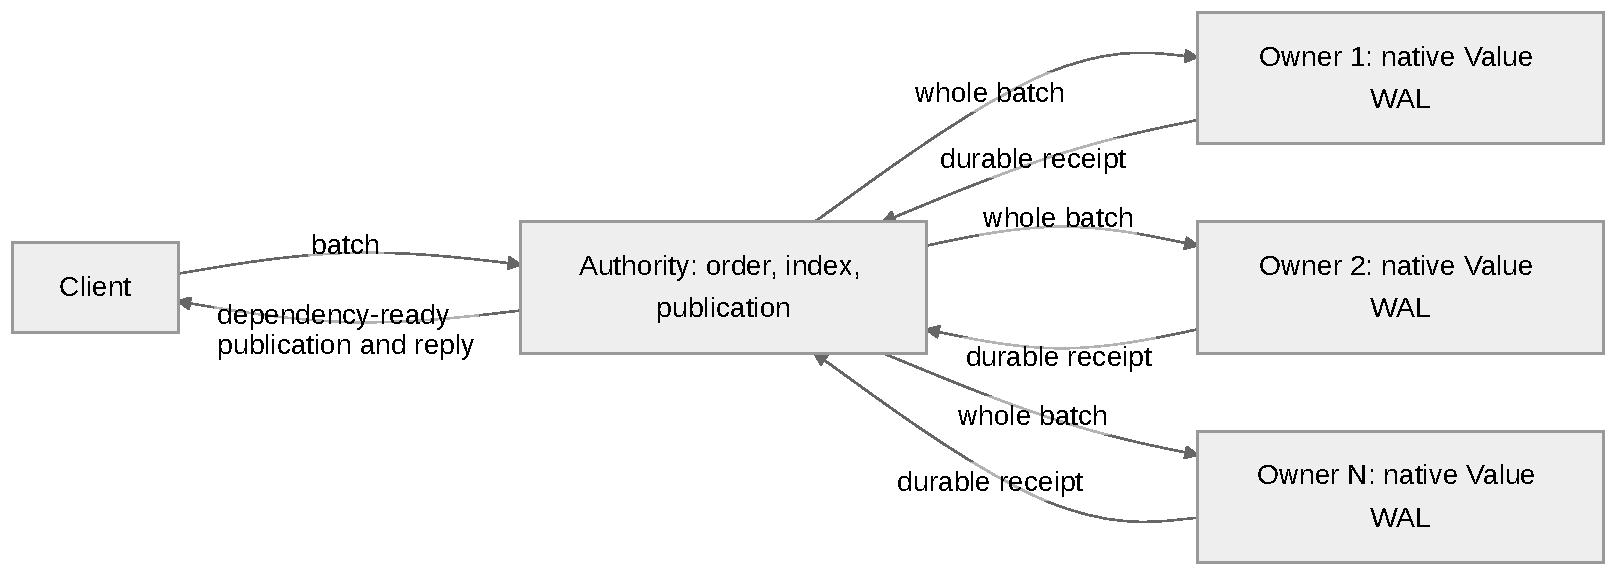
\includegraphics[width=.97\linewidth,height=2.05in,keepaspectratio]{figures/topology.pdf}\\[-2pt]
\small Figure 1. A complete batch goes to one owner and receives one durable receipt. Each owner maintains its own Value WAL; arrows do not represent replication.
\end{center}

The coordinator, called the authority in the code, reserves capacity, assigns a logical batch version and selects an owner. That owner appends and persists the complete batch. The coordinator publishes the corresponding index updates after relevant predecessors resolve. Successive updates to a key can reside on different owners. Logical versions order updates; they are not offsets in a global physical log.

Independent durable batches can become visible while an unrelated earlier batch is unresolved. Updates sharing an index identity respect their dependencies. A stable checkpoint frontier advances only through a contiguous resolved prefix; retained read views pin the history needed for their cuts. Reduced-key collisions can make distinct full keys interfere. Separate batches can overlap in storage, while shared coordinator state and native locks protect admission and publication.

The measured configuration has one durable owner per batch (RF1). Recovery fences old writers and reconciles available inventories and durable records, including uncertain requests with lost replies. Permanent loss of an owner's only copy is not tolerated. The prototype does not provide consensus-backed failover or general serializable transactions across independent logical databases; distributed live-value relocation is not complete.

\section*{3. Read paths and measurement contract}
\begin{center}
\small
\fbox{Index reference at coordinator}
$\longrightarrow$
\fbox{\begin{tabular}{c}Optional validated\\coordinator-cache hit\end{tabular}}
\quad or \quad
\fbox{\begin{tabular}{c}Owner WAL read\\(possibly page-cached)\end{tabular}}\\[4pt]
\small Figure 2. Current read alternatives after index lookup: a validated coordinator-cache hit or a request to the owner WAL.
\end{center}

A validated coordinator-cache hit avoids owner data traffic while authority health is checked. Otherwise the exact reference routes a request to its owner. The current path has no explicit owner application value cache: the WAL read may be served by Linux page cache or require storage I/O. The presence of a verbs transport does not establish a one-sided read or physical device access.

The campaign used six \texttt{z4m-highmem-16} VMs in \texttt{us-central1-a}: one coordinator and five storage hosts, each with its own Local SSD allocation. Placement was compact, with maximum distance 3; management used GVNIC and the RDMA interfaces used IRDMA/Falcon. Cross-host RDMA READ/SEND and Valkey RDMA operations were qualified before measurement. Falcon is the Google Cloud transport in this comparison, not AWS EFA.

The workload covers 64 B, 256 B, 1 KiB, 8 KiB and 64 KiB values, point and 32-value reads, writes, mixed operations, uniform and Zipf reads, and offered-load cases. Primary RF1 Tidehunter cases disable the coordinator value cache; Linux page cache remains available. Separate campaign cohorts configure coordinator caches and attempt cold-OS-cache eviction. Cold OS cache does not guarantee physical SSD access or remove private engine caches; Valkey values remain RAM-resident. These cohorts are distinct from the primary cases.

The ten arms are native Tidehunter, distributed Tidehunter TCP and Falcon/verbs, Valkey TCP and RDMA, Garnet, Kvrocks, Cassandra, TiKV and FoundationDB. RF1 aligns replica count, not consistency, durability, transaction, security or failure guarantees. Native uses one host rather than a coordinator and five storage hosts. Native and distributed Tidehunter use the specified Value-WAL barrier; other stores retain their own exported contracts. Adapter operations also differ, including the implementation of multi-value reads.

API latency measures dispatch to completion. Scheduling delay precedes dispatch; response latency runs from scheduled arrival to completion and thus includes that delay. Successful-operation latency excludes rejected arrivals, which remain in the offered-load accounting. Each case has one independent repetition; the observed percentiles and within-case standard deviations do not estimate run-to-run variability. No confidence intervals or significance claims follow from this campaign.

\section*{4. Matched backend comparison}
Table 1 shows successful API-call latencies for separate primary RF1, concurrency-16 cases at 1 KiB. A read-32 latency covers the complete request, not an individual value. The source populations contain 8,192 reads, 4,096 writes and 2,048 read-32 calls per case. The reported p99 is descriptive of these samples.

\begin{center}
\small
\begin{tabular}{lrrrrr}
\toprule
Backend & Read p50 & Read p99 & Write p50 & Write p99 & Read-32 p50 \\
 & \multicolumn{5}{c}{API latency (\us)} \\
\midrule
Native Tidehunter & 1.58 & 2.56 & 189.34 & 304.79 & 58.84 \\
Tidehunter TCP & 66.72 & 269.74 & 357.69 & 8,411.26 & 2,395.62 \\
Tidehunter Falcon/verbs & 38.63 & 180.80 & 337.95 & 8,824.48 & 2,144.30 \\
Valkey TCP & 49.35 & 112.07 & 170.96 & 430.73 & 356.46 \\
Valkey RDMA & 36.84 & 55.47 & 166.24 & 397.09 & 273.19 \\
Garnet & 84.10 & 124.77 & 140.08 & 63,619.97 & 2,230.42 \\
Kvrocks & 84.11 & 123.34 & 255.51 & 897.90 & 1,981.36 \\
Cassandra & 92.24 & 167.97 & 299.84 & 1,311.12 & 1,932.36 \\
TiKV & 191.18 & 318.43 & 277.44 & 549.91 & 3,633.67 \\
FoundationDB & 276.80 & 398.37 & 986.47 & 1,224.14 & 5,053.06 \\
\bottomrule
\end{tabular}\\[3pt]
Table 1. Matched 1 KiB successful operations; one repetition. Case-level data and all timing clocks are recorded in \texttt{evidence.json}.
\end{center}


\begin{center}
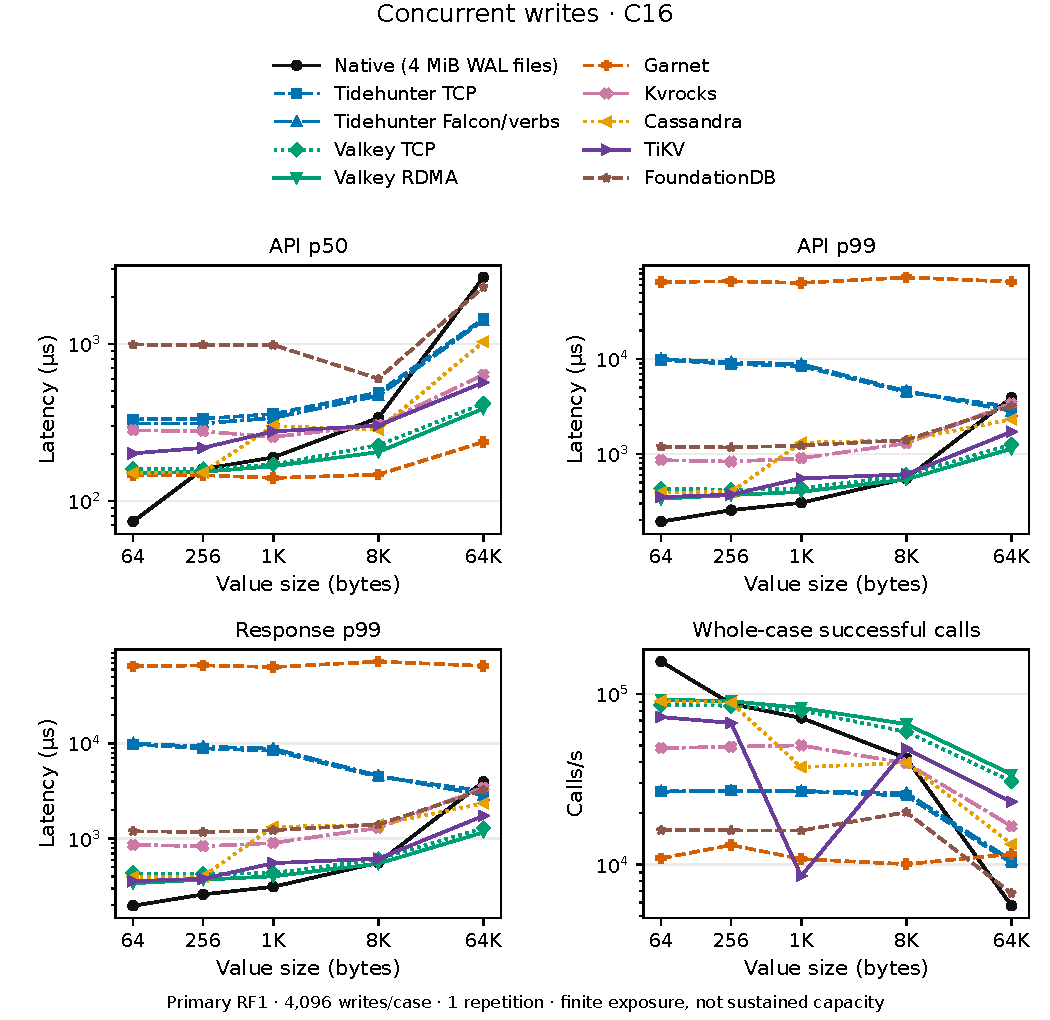
\includegraphics[width=\linewidth]{figures/gcp-primary-write-concurrent.pdf}\\[-2pt]
\small Figure 3. Primary concurrent scalar writes across five value sizes: successful API p50 and p99, response p99, and whole-case successful calls/s. Both value size and latency/rate axes are logarithmic. Each point contains 4,096 measured writes and one repetition; there are no between-run error bars.
\end{center}
The table does not establish a universal ranking. An in-process native lookup on the cloud host avoids a remote request, while a distributed miss must cross process and machine boundaries and complete routing, service and validation; even a warm page-cache hit does not eliminate those costs. Falcon has a lower Tidehunter point-read median than TCP here and is close to Valkey RDMA, but transport labels do not isolate the network from protocol, scheduling, copying, security or storage differences. At concurrency one in a separate 1 KiB mixed case, successful read medians were 1.113 \us\ native, 44.575 \us\ TCP and 26.527 \us\ verbs; these samples must not be pooled with the concurrency-16 cases.

Both Valkey arms observed AOF enabled with \texttt{appendfsync=always}; their write results must not be explained as nonpersistent memory-only acknowledgements. Tidehunter's WAL receipt and publication use a different persistence path. At 1 KiB, Tidehunter verbs has a 338 \us\ median and 8.82 ms p99, while Garnet combines a 140 \us\ median with a 63.62 ms p99. These complete-operation latencies do not isolate transport. Tidehunter TCP used mutual TLS, while the verbs path used trusted-network transport without TLS.

\begin{center}
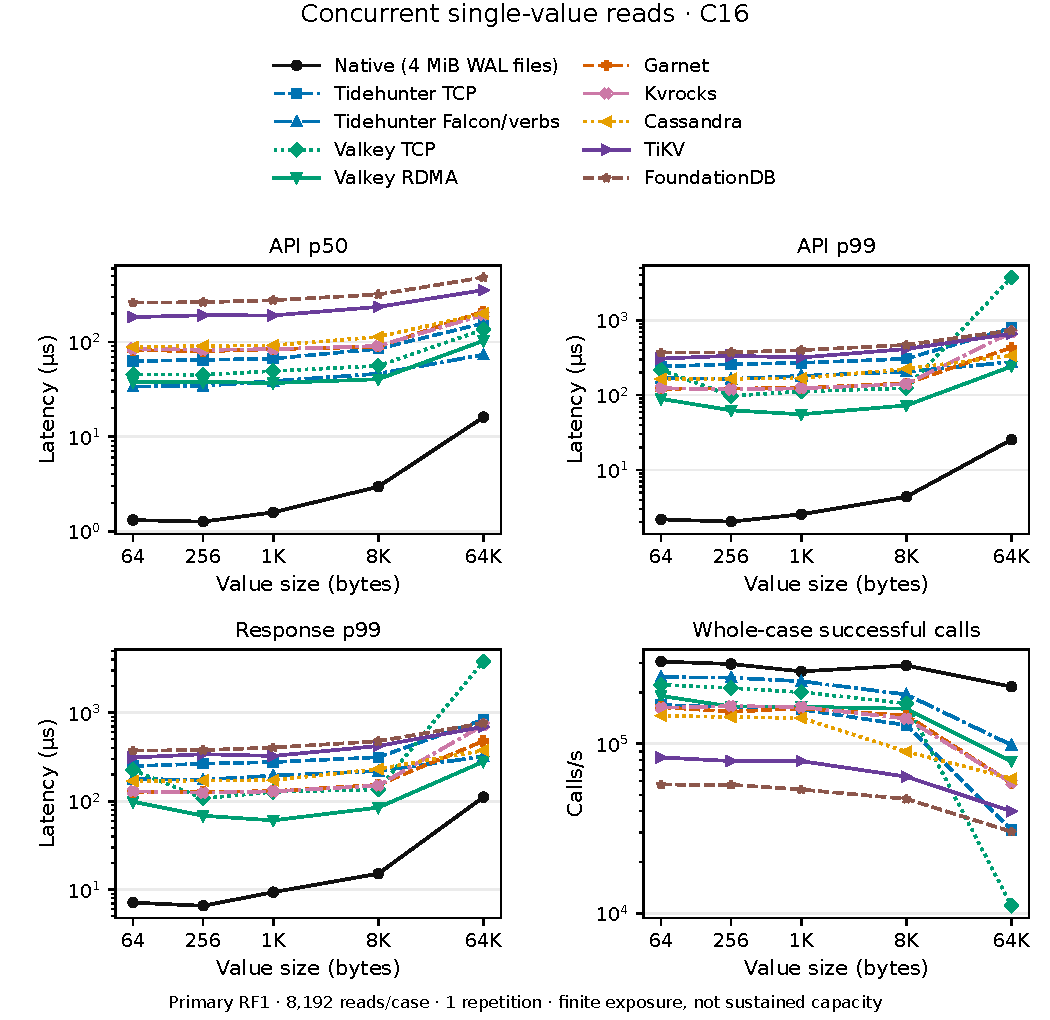
\includegraphics[width=\linewidth]{figures/gcp-primary-read-concurrent.pdf}\\[-2pt]
\small Figure 4. Primary concurrent single-value reads across five value sizes: successful API p50 and p99, response p99, and whole-case successful calls/s. Both axes are logarithmic. Each point contains 8,192 measured reads and one repetition; there are no between-run error bars.
\end{center}

\section*{5. Cache, batches and load}
In separate coordinator-cache-configured cohorts, TCP read API medians were 0.538 \us\ for 256 B and 0.598 \us\ for 8 KiB; Falcon/verbs medians were 0.525 and 0.692 \us. The 8 KiB verbs counter receipt records cache hits, zero misses and zero read RPCs. These coordinator-cache measurements from the cloud campaign are not remote-read latency and are not a controlled estimate of the cache benefit alone.

The 32-value read results remain much farther from Valkey than the point-read medians: at 1 KiB the complete Tidehunter verbs call is 2,144.30 \us\ versus 273.19 \us\ for Valkey RDMA. A batch returns all 32 results, so its critical path includes grouping, progress and completion of its slowest required work; it is not a single-value latency multiplied or divided into an equivalent point read. The implementations and their memory-residency and API semantics differ. At 8 KiB the complete batch median was 97.074 \us\ native, 2,285.889 \us\ Tidehunter TCP, 2,328.105 \us\ Tidehunter verbs and 304.934 \us\ Valkey RDMA. One repetition cannot establish the cause of the gap or a TCP/verbs regression, nor separate coordination, network and storage time.

All 6,262,400 offered calls were accounted for, including 323,195 rejected arrivals in overloaded cases. At the requested 50,000 calls/s, Tidehunter TCP completed 43,892 calls/s with 48,668 rejected arrivals; verbs completed 44,454 calls/s with 44,291 rejected arrivals. Valkey RDMA had 1,385 rejected arrivals. These bounded exposures are not an indefinitely sustainable throughput limit. Successful-call latency alone omits rejected arrivals.

\section*{6. Interpreting the write curves}
The native 64 KiB median is 2,652.295 \us, compared with 337.753 \us\ at 8 KiB: 7.85 times the latency for eight times the value bytes. Its successful value-payload rate increases from 328.54 to 358.65 MiB/s. The calls/s decrease is therefore not a decrease in value bandwidth. The increase affects the distribution broadly, rather than arising from one extreme sample.

The native benchmark uses Tidehunter's small configuration: 1 MiB fragments and 4 MiB WAL files. Each scalar put explicitly waits for a Value-WAL barrier that synchronizes all registered files and the directory. The distributed owner uses 4 MiB fragments and 1 GiB files. This is a configuration difference worth testing, not evidence that the historical native result should be replaced. The Tidehunter paper's 830K writes/s at 1 KB used a different machine, a 1 TB fill and ten-minute measurements; its normal foreground write does not wait for fsync. It is not the acknowledgement contract measured here.

TiKV's 1 KiB throughput dip comes from a recorded pause: 16 of 4,096 calls take 398.61--406.01 ms, with a 398.357 ms gap between completions. Their 0.39\% share leaves p99 near 550 \us\ while p99.9 reaches 404.69 ms. The whole case lasts 477.855 ms, so the 8,572 calls/s point faithfully includes that pause. All primary write exposures are only 26.4--713.8 ms; these points must not be presented as sustained capacity or a reproducible size-dependent TiKV ranking.

\begin{center}
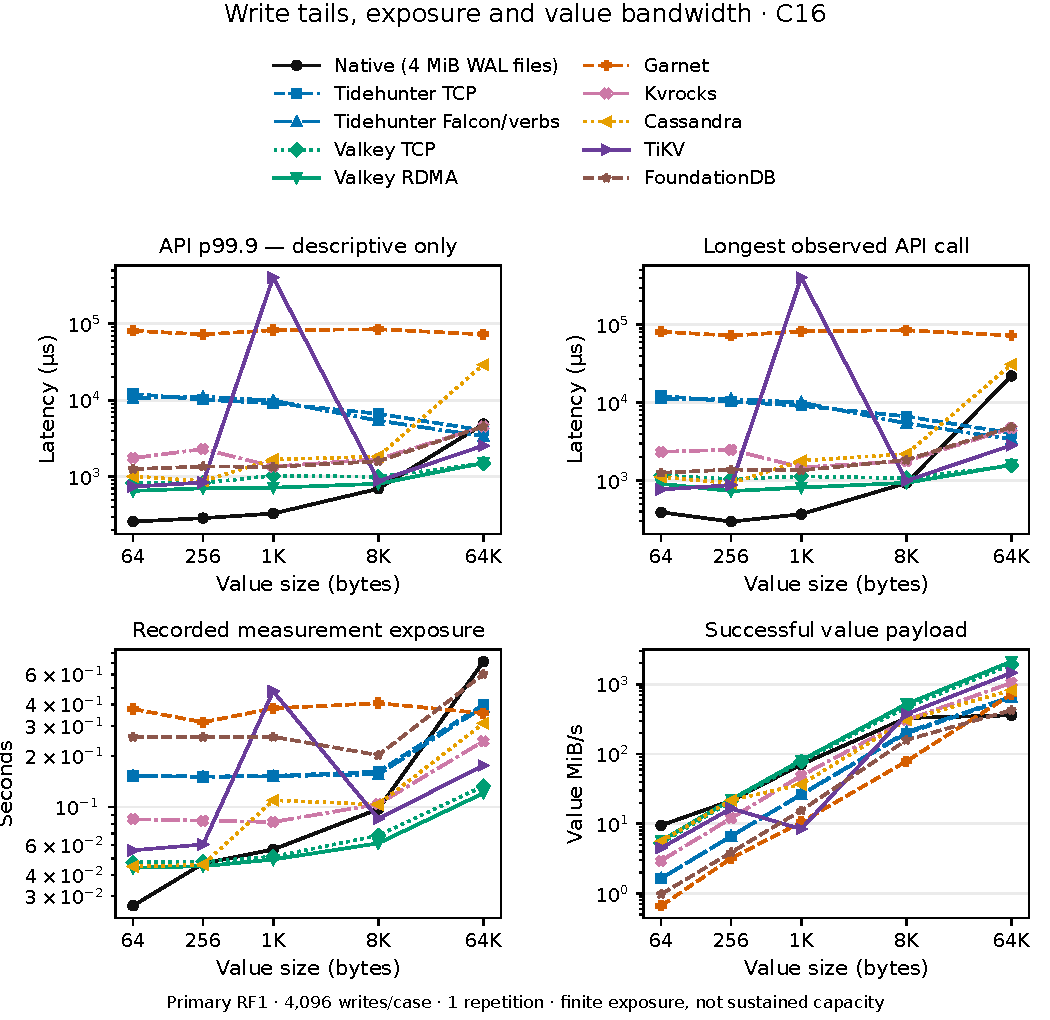
\includegraphics[width=\linewidth]{figures/gcp-write-diagnostics.pdf}\\[-2pt]
\small Figure 5. The same cloud write cases, exposing descriptive p99.9, maximum latency, measurement duration and successful value-payload bandwidth. No samples were removed and no new campaign was run.
\end{center}

Receive-buffer exhaustion is a valid RDMA tail-latency hypothesis, but these cases do not measure hardware receive credits or RNR retries. Tidehunter's selected provider is \texttt{verbs;ofi\_rxm}; its four application receive slots are not four hardware receive WQEs. Separate 1 KiB write-diagnostic cases record seven foreground admission-pressure episodes in both transports, totaling 56.30 ms for verbs and 50.67 ms for TCP. Those spans include draining and checkpoint waiting, not just persistence. This identifies a shared candidate for investigation, not a per-request attribution of Figure 3's tails. Buffer sizing and admission pressure must be separated before changing either.


\clearpage

\section*{7. Sources and reproducibility}
The distributed code is under \path{tidehunter/src/distributed/}: \path{sequence.rs} and \path{types.rs} distinguish logical versions and addresses; \path{storage.rs} handles owner WAL operations; \path{remote_db.rs}, \path{publication.rs} and \path{native_index/retention.rs} cover admission and visibility. The benchmark harness is under \path{experiments/kv-comparison/} and \path{benchmarks/kv-research/}. The Mermaid source for Figure 1 remains in \path{architecture.mmd}.

Campaign \texttt{bench-b35a62e24b47faaf} used frozen source SHA-256 \path{98cc1eb67e1d2c269294a391acf0bcdfc9ef029813ef348a89e92939f10d6c0a} and benchmark binary SHA-256 \path{34bb9d91cf9bf3c2e343827cd20ee8b1526cdcd764bc16800c4c54476de1c065}. These are content digests, not Git commit identifiers. The campaign report, original comparison JSON, 1,446-row all-populations CSV, figure manifest, raw archive and cleanup receipt are identified in the accompanying README and \path{evidence.json}. The CSV retains available p50, p95, p99, p99.9, mean, standard deviation and maximum for API, scheduling and response clocks, without turning absent clocks into zeros. Figures 3--5 are generated by \path{plot_evidence.py} from the campaign comparison JSON; the evidence record identifies every plotted case and source value.

The six VMs, boot disks and placement policy were confirmed deleted at 04:56:38 UTC on 3 November. The archived source and binary are the measured cloud artifacts. No AWS data are pooled with this GCP campaign.

\begin{thebibliography}{9}\small
\bibitem{tidehunter} A. Chursin et al., \emph{Tidehunter: Large-Value Storage With Minimal Data Relocation}, 2026, \href{https://arxiv.org/abs/2602.01873v2}{arXiv:2602.01873v2}.
\end{thebibliography}
\end{document}
